\documentclass[final,t]{beamer}
\setbeamersize{text margin left = 25pt, text margin right = -5pt}

\usepackage{graphicx}

\usepackage{resizegather}

% poster template
% \usepackage[orientation=landscape,size=a0,scale=1.4,debug]{beamerposter}
\usepackage[orientation=landscape,size=a0,scale=1.3,debug]{beamerposter}
% \usepackage[orientation=landscape,size=custom,width=160,height=100,scale=1.8,debug]{beamerposter}
% \usepackage[ruled, vlined]{algorithm2e}
\usetheme{combined}
% \usefonttheme{default}
\usefonttheme[onlymath]{serif}

% references backend=biber, style=alphabetic, citestyle=authoryear, ,hyperref=auto
\usepackage[backend=biber,bibstyle=authoryear,citestyle=authoryear-comp]{biblatex}
\bibliography{./bibliography}

% private packages
\usepackage{tikz}
\usetikzlibrary{arrows,decorations.pathmorphing,backgrounds,positioning,fit,petri,mindmap,shapes.geometric, shapes.misc}
\tikzset{cross/.style={cross out, draw=black, minimum size=2*(#1-\pgflinewidth), inner sep=0pt, outer sep=0pt},
%default radius will be 1pt.
cross/.default={1pt}}
\usepackage{color}
\usepackage{hyperref}       % hyperlinks
\usepackage{url}            % simple URL typesetting
\usepackage{booktabs}       % professional-quality tables
\usepackage{nicefrac}       % compact symbols for 1/2, etc.
\usepackage{microtype}
%\usepackage{amssymb}
\usepackage{amsmath}
%\usepackage{amsthm}
% \usepackage{amsfonts}
\usepackage{algorithm, algpseudocode}%,algorithmic}
% \usepackage[square,numbers]{natbib}
% \usepackage{natbib}
\usepackage{wrapfig}
\usepackage{subcaption}
% \usepackage{bibentry}
% \bibliography{../bibfile}
\usepackage{listings}
\lstdefinestyle{customc}{
  %belowcaptionskip=1\baselineskip,
  breaklines=true,
  language=C,
  showstringspaces=false,
  basicstyle=\footnotesize\ttfamily,
  keywordstyle=\bfseries\color{black!40!black},
  identifierstyle=\color{black}
}

\lstset{style=customc}
\usepackage{xcolor}

\floatname{algorithm}{Algorithm}
\renewcommand{\algorithmicrequire}{\textbf{Input:}}
\renewcommand{\algorithmicensure}{\textbf{return}}
\renewcommand{\algorithmicfunction}{\textbf{def}}
\algtext*{EndFunction}

\definecolor{vectorpink}{HTML}{E40086}


% -------------------- Math macros -----------------------------
%\newcommand{\norm}[1]{||#1||}
\newcommand{\etal}{\textit{et al}.}
%\newcommand{\TODO}[1]{{\color{red}TODO: #1}}
%\newcommand{\NOTE}[1]{{\color{blue}NOTE: #1}}
% \newtheorem{theorem}{Theorem}
\newtheorem*{theorem*}{Theorem}
\newtheorem*{lemma*}{Lemma}
\newcommand{\tr}{\textnormal{tr}}
\newcommand\E{\mathbb{E}}
\newcommand\R{\mathbb{R}}
%\newcommand{\B}{\mathbb{B}}
%\newcommand{\A}{\mathbb{A}}
% overwrite epsilon as varepsilon
\renewcommand{\epsilon}{\varepsilon}
%\newcommand*{\matr}[1]{\mathbfit{#1}}
\newcommand*{\tran}{^{\mkern-1.5mu\mathsf{T}}}
%\newcommand*{\conj}[1]{\overline{#1}}
%\newcommand*{\hermconj}{^{\mathsf{H}}}

\newcommand{\vx}{\mathbf{x}}
\newcommand{\vepsilon}{\mathbf{\epsilon}}
\newcommand{\vtheta}{\mathbf{\theta}}%
\newcommand{\vpsi}{{\bm{\psi}}}
\newcommand{\vpi}{{\bm{\pi}}}
\newcommand{\vphi}{{\bm{\phi}}}
\newcommand{\vz}{\mathbf{z}}
\newcommand{\vX}{\mathbf{X}}
\newcommand{\vw}{\mathbf{w}}
\newcommand{\vv}{\mathbf{v}}
\newcommand{\vr}{\mathbf{r}}
\newcommand{\vh}{\mathbf{h}}
\newcommand{\vg}{\mathbf{g}}
\newcommand{\vI}{\mathbf{I}}
\newcommand{\vzero}{{\bf{0}}}
\newcommand{\ones}[1]{\mat{1}_{#1}}
\newcommand{\eye}[1]{\mat{E}_{#1}}
\newcommand{\tra}{^{\mathsf{T}}}
\newcommand{\vect}[1]{{\bf{#1}}}
\newcommand{\mat}[1]{\mathbf{#1}}
\newcommand{\pderiv}[2]{\frac{\partial #1}{\partial #2}}
\newcommand{\npderiv}[2]{\nicefrac{\partial #1}{\partial #2}}
\newcommand{\argmin}{\operatornamewithlimits{argmin}}
\newcommand{\argmax}{\operatornamewithlimits{argmax}}
\newcommand{\expect}{\mathbb{E}}
\newcommand{\expectargs}[2]{\mathbb{E}_{#1} \left[ {#2} \right]}
\newcommand{\var}{\mathbb{V}}
\newcommand{\varL}{\mathcal{L}}
\def\iid{i.i.d.\ }
\def\simiid{\overset{\mbox{\tiny iid}}{\sim}}
\newcommand{\defeq}{\mathrel{:\mkern-0.25mu=}}
\newcommand{\Normal}{\mathcal{N}}
\newcommand{\Nt}[3]{\mathcal{N}\!\left(#1 \middle| #2,#3\right)}
\newcommand{\N}[2]{\mathcal{N}\!\left(#1,#2\right)}
\DeclareMathOperator{\KLop}{KL}
\newcommand{\KL}[2]{\KLop \left(#1 \middle \| #2 \right)}
\newcommand{\tunderbrace}[1]{\underbrace{\textstyle #1}}

\newcommand{\norm}[2][]{#1\lVert #2 #1\rVert}

%%%%%%%%%%%% Vectors %%%%%%%%%%%%%%
\def\ve#1{\mathchoice{\mbox{\boldmath$\displaystyle\bf#1$}}
{\mbox{\boldmath$\textstyle\bf#1$}}
{\mbox{\boldmath$\scriptstyle\bf#1$}}
{\mbox{\boldmath$\scriptscriptstyle\bf#1$}}}

%%%%%%%%%% Bold face letters  %%%%%%%%%%%%%
\newcommand{\rx}{{\ve r}}
\renewcommand{\u}{{\ve u}}
\newcommand{\x}{{\ve x}}
\newcommand{\w}{{\ve w}}
\newcommand{\A}{\textrm{A}}
\newcommand{\B}{\textrm{B}}

% -------------------- Define notation here --------------------

\newcommand{\latent}{\vz}
\newcommand{\hidden}{\vh}
\newcommand{\obs}{\vx}
\newcommand{\sol}{\vz}  % Solution to ODE (normally x or y}
\newcommand{\obsdim}{D_x}
\newcommand{\latentdim}{D}
\newcommand{\solvefunc}{\text{ODESolve}}
\newcommand{\tstart}{{t_\text{0}}}
\newcommand{\tend}{{t_\text{1}}}
\newcommand{\lograte}{\lambda}%\text{lograte}}
\newcommand{\method}{Latent ODE}
\newcommand{\cnfx}{\sol}


% document properties
\title{Nesterov's Accelerated Gradient Descent's Speed}
\author{\Large Joshua Tan, Manoj Manikandan, Rohan Navaratnam}
\institute{Department of Computer Science, University of Manchester}


\begin{document}

\begin{frame}[containsverbatim]

\begin{columns}[t]

%-------------------------------------------------------------                          
%COLUMN 1
% ------------------------------------------------------------

\begin{column}{.32\linewidth}
    \vspace{-18mm}
    
    \begin{exampleblock}{Introduction}
    Recent works like \cite{dziugaite2017computing} and \cite{zhou2018non} have shown that one can obtain non-vacuous ``computational" PAC-Bayesian bounds on the risk of neural nets. In this work we improve on existing theoretical PAC-Bayesian risk bounds by using data-dependent priors sensitive to the geometrical properties of training and by considering carefully chosen clusters of multiple nets in tandem.  
    
    % These experiments strongly motivate the current work to search for stronger theoretical basis towards explaining the power of PAC-Bayesian risk bounds in explaining the generalization ability of neural nets. Previous PAC-Bayes bounds (and us too) have used data dependent priors on the geometric mean of the spectral norms of the layer matrices to try to track the first parameter above. In this work we also propose a mechanism of choosing the finite set priors in such a way that can also track the angular deflection in a data-dependent way. 

    % {\it Secondly,} we go further to show how in the PAC-Bayesian framework one can leverage more out of the angle parameter by simultaneously training a clusters of nets that is by obtaining in tandem a finite set of classifiers/neural functions on the chosen architecture by simultaneously training multiple instances initialized at different by closeby weight vectors. Because of this use of clusters, compared to previous bounds our dependency on the distance from initialization is also more intricate and we are able to get more sensitive to the average case behaviour. Thus we build into the theory more data-dependent (and hence tunable) parameters which help us further improve over existing bounds. And to incorporate the effect of the cluster we need to prove new noise resilience theorems for neural nets. 
    \end{exampleblock}
    
    % \begin{exampleblock}{TO DO}
    % Hello! 
    % \end{exampleblock}


    \begin{exampleblock}{Notation}
      \begin{itemize}
      \item $\delta f(x)$ is the set of \textbf{subgradients} of the point $x \in \mathbb{R}^n$. Then the subgradient $g \in \delta f(x)$ satisfies $f(x) - f(y) \leq g^\top (x-y)$.
      \item $e_1, \dots, e_n$ is the canonical basis of $\mathbb{R}^n$.
      \item $x^* \in \mathbb{R}^n$ is a point such that it is the minima in any optimisation problem, i.e. $f(x^*) = \mathop{\min}\limits_{x \in \mathbb{R}^n} f(x)$. 
      We always assume $x^*$ exists.
      \item $\norm{\cdot}$ is always the Euclidean norm $\norm{x} = \sqrt{x_1^2 + x_2^2 + \dots + x_n^2}$ for $x \in \mathbb{R}^n$
      \end{itemize}
    \end{exampleblock}
   \begin{exampleblock}{Fastest theoretical speed for Gradient Descent}
    \begin{theorem}[{\bf 1}] \label{thm:3.14}
      Let $t \leq \frac{n-1}{2}$ and $\beta > 0$. There exists a $\beta$-smooth convex function $f$ such that for any black-box procedure satisfying 
      $x_{t+1} \in \text{Span}(g_1, \dots, g_t)$ with $g_s \in \delta f(x_s)$:
      \begin{equation*}
        \mathop{\min}\limits_{1 \leq s \leq t} f(x_s) - f(x^*) \geq \frac{3\beta}{32} \frac{\norm{x_1 - x^*}^2}{(t + 1)^2}
      \end{equation*}
    \end{theorem}
    \begin{center}
      \textcolor{red}{This gives us a bound on the speed of gradient descent of $O(1/t^2)$. We observe that this bound is achieved by Nesterov's Accelerated Gradient Descent}
    \end{center}
    \end{exampleblock}
    
    \begin{exampleblock}{Crafting a $\beta$-smooth function $f$}
      To construct a suitable function $f$ that satisfies Theorem (\ref{thm:3.14}), Bubeck constructs a symmetric and tri-diagonal matrix
      \begin{equation*}
        (A_k)_{i,j} = \begin{cases}
          2, \ &i=j \ , \ i \leq k \\
          -1, \ &j \in \{i - 1, i + 1\}, \ i \leq k, \ j \neq k + 1 \\
          0, &\text{ otherwise}
        \end{cases}
      \end{equation*}
      and defines $f$ as:
      \begin{equation*}
        f(x) = \frac{\beta}{8}x^\top A_{2t + 1}x - \frac{\beta}{4}x^\top e_1
      \end{equation*}
      
    \end{exampleblock}
    \begin{exampleblock}{References}
    %\small 
        \vspace{1mm} 
    \printbibliography
    \vspace{1mm} 
    \end{exampleblock}
\end{column}


%-------------------------------------------------------------------------         
%COLUMN 2
% ------------------------------------------------------------------------


\begin{column}{.32\linewidth}
\vspace{-18mm}







\begin{exampleblock}{Descent Lemma}
The following lemma establishes the per-step bound for gradient descent on smooth functions. The original 
paper states the constrained case but for Nesterov's accelerated gradient descent in the smooth 
function case, we only need the unconstrained version.
\begin{lemma}[\bf 2]\label{lemma:3.6}
Let $f:\mathbb{R}^n \rightarrow \mathbb{R}$ be a convex and $\beta$-smooth function. Let $x, y \in \mathbb{R}^n$ and $x^+ = x - \frac{1}{\beta}\nabla f(x)$.
Then the following holds true:
\begin{equation*}
  f(x^+) - f(y) \leq \nabla f(x)^\top (x - y) - \frac{1}{2\beta}\norm{\nabla f(x)}^2
\end{equation*}
\end{lemma}
\end{exampleblock}




\begin{exampleblock}{Nesterov's accelerated gradient descent}

    \begin{figure}
      \begin{center}
        \begin{tikzpicture}[scale=2.5]
          \node [tokens=1] (noeud1) at (0.5,1) [label=below right:{$x_s$}] {};
          \node [tokens=1] (noeud2) at (1.5,-1) [label=below right:{$y_{s}$}] {};
          \node [tokens=1] (noeud3) at (2.5,2) [label=below right:{$y_{s+1}$}] {};
          \node [tokens=1] (noeud4) at (2.8,3) [label=above left:{$x_{s+1}$}] {};
          \draw[->, thick] (noeud1) -- (noeud3) node[midway, left, xshift=-0.3cm] {$-\frac{1}{\beta}\nabla f(x_s)$};
          \draw[thick, dashed] (noeud2) -- (noeud4) {};
          \node [tokens=1] (noeud5) at (4.5,3.3) [label=below right:{$y_{s+2}$}] {};
          \node [tokens=1] (noeud6) at (5.3,3.8) [label=right:{$x_{s+2}$}] {};
          \draw[->, thick] (noeud4) -- (noeud5) {};
          \draw[thick, dashed] (noeud3) -- (noeud6) {};
        \end{tikzpicture}
        \end{center} 
      \caption{Illustration of Nesterov's accelerated gradient descent.}
      \label{fig:nesterovacc}
    \end{figure}
    First we introduce the following sequences:
    \begin{equation*}
      \lambda_0 = 0, \ \lambda_t = \frac{1 + \sqrt{1 + 4\lambda_{t-1}^2}}{2}, \ \text{and} \ \gamma_t = \frac{1 - \lambda_t}{\lambda_{t + 1}}
    \end{equation*}
    Nesterov's accelerated gradient descent is described as follows. Start at an arbitrary initial point $x_1=y_1$ and then iterate 
    the following equations for $t\geq1$
    \begin{align}
    y_{t+1} &= x_t - \frac{1}{\beta}\nabla f(x_t) \label{nesterov:y}\\  % <-- label fixed
    x_{t+1} &= (1 - \gamma_t)y_{t+1} + \gamma_t y_t \label{nesterov:x}  % <-- label fixed, sign fixed
    \end{align}
    Nesterov's accelerated gradient descent uses the ideas from classical momentum gradient descent (\cite{sutskever}). 
    $x_{t+1}$ can be rewritten as $x_{t+1} = y_{t+1} - \gamma_t(y_{t+1} - y_{t})$ which reads as $x_{t+1}$ overshoots $y_{t+1}$ along the vector 
    $(y_{t+1} - y_{t})$ with some ``momentum'' given by $\gamma_t$ % <-- sign fixed (- instead of +)
    \begin{theorem}[{\bf 3}]
    Let $f$ be a convex and $\beta$-smooth function, then Nesterov's accelerated gradient descent satisfies
    \newline \\
    \begin{equation*}
      f(y_t) - f(x^*) \leq \frac{2\beta\norm{x_1 - x^*}^2}{t^2}
    \end{equation*}
    \end{theorem}

    This gives us the $O(1/t^2)$ complexity. \textcolor{red}{Write more about it here}
    \end{exampleblock}

    \end{column}


    %------------------------------------------
    %Column 3
    %------------------------------------------

    \begin{column}{.32\linewidth}
    \vspace{-18mm}

    \begin{exampleblock}{Key insights from Proof of Theorem $3$}
    \begin{itemize}
      \item We can reverse engineer both $\lambda_t$ and $\gamma_t$ to show they are not arbitrary. If we rewrite (\ref{nesterov:x}) as $x_{t} = y_{t} + d_t$ 
      where $d_t = \gamma_t (y_{t} - y_{t-1})$ is the momentum term and 
      let $g_{t} = -\frac{1}{\beta}\nabla f(y_{t} + d_t)$ be the gradient term in $y_{t+1}$ by rewriting $x_t$ as above (\ref{nesterov:y}), we get the following two 
      inequalities when applying Lemma~\ref{lemma:3.6}:
      \begin{align*}
        f(y_{t+1}) - f(y_t) &\leq -\frac{\beta}{2}(\norm{g_t}^2 - 2g_t \cdot d_t)  \tag{$\star$} \label{ineq:1}\\
        f(y_{t+1}) - f(x^*) &\leq -\frac{\beta}{2}(\norm{g_t}^2 - 2g_t \cdot (x_t + d_t - x^*)) \tag{$\star\star$} \label{ineq:2} % <-- x_y -> x_t
      \end{align*}
      \item The big idea is to use the identity $\norm{a}^2 + 2ab = \norm{a+b}^2 - \norm{b}^2$ on the combination of both inequalities to obtain a telescopic sum~\cite{BubeckUpdatePost}. 
      Let $\delta_t = f(y_{t}) - f(x^*)$. Then by multiplying (\ref{ineq:1}) by $(\lambda_t - 1)$ and adding (\ref{ineq:2}) we obtain:
      \begin{align*}
      \lambda_t \delta_{t+1} - (\lambda_t - 1)\delta_t
        &\leq -\frac{\beta}{2} \bigl(\lambda_t \|g_t\|^2 + 2\, g_t \cdot(x_t + \lambda_t d_t - x^*)\bigr) \\
        &= -\frac{\beta}{2}\frac{1}{\lambda_t} \bigl(\|x_t + \lambda_t d_t - x^* + \lambda_t g_t\|^2 \\
        &\phantom{{}= -\frac{\beta}{2}\frac{1}{\lambda_t} \bigl(}
          - \|\,x_t + \lambda_t d_t - x^*\|^2\bigr) \tag{$\dagger$} \label{eq:1}
    \end{align*}
      where the equality comes by applying the identity with $a = \lambda_t g_t$ and $b = x_t + \lambda_t d_t - x^*$.
      \item To obtain the telescopic sum, we need
      \begin{equation*}
        x_t + \lambda_t d_t - x^* + \lambda_t g_t = x_{t+1} + \lambda_{t+1} d_{t+1} - x^*
      \end{equation*}
      which comes from observing (\ref{eq:1}). Since $d_{t+1} = x_{t+1} - y_{t+1} = -\gamma_t (d_t + g_t)$ and $x_{t+1} = x_t + g_t + d_t$: % <-- gamma_{t+1} -> -gamma_t
      \begin{align*}
        x_t + \lambda_t d_t - x^* + \lambda_t g_t &= x_t + g_t + d_t - \lambda_{t+1} \cdot \gamma_t (g_t + d_t) - x^* \\ % <-- sign and index fixed
        \lambda_t (d_t + g_t) &= (d_t + g_t)(1 - \lambda_{t+1}\cdot\gamma_t) % <-- sign and index fixed
      \end{align*}
      and hence $\gamma_t = \frac{1 - \lambda_t}{\lambda_{t+1}}$ % <-- gamma_{t+1} -> gamma_t
      \item Now to select $\lambda_t$, by multiplying $\lambda_t$ to (\ref{eq:1}) and denoting $u_t := \frac{\beta}{2}\norm{x_t + \lambda_t d_t - x^*}$ we get
      \begin{equation*}
        \lambda_t^2 \delta_{t+1} - (\lambda_t^2 - \lambda_t)\delta_t \leq u_t - u_{t+1}
      \end{equation*}
      and therefore $\lambda_t^2 - \lambda_t = \lambda_{t-1}^2$ is required to obtain the full telescopic sum. The rest of the proof follows by induction.
    \end{itemize}
    \end{exampleblock}


\begin{exampleblock}{Demonstration of stability of the relevant geometrical properties of training}
\vspace{2.2mm}
In the {\it \color{violet} figure to the left} we plot the initial parameter norm $\norm{\B}_2$ vs the final parameter norm $\norm{\A}_2$ for training nets of different depths at width $100$ on the CIFAR-10 dataset. Thus its demonstrated that the multiplicative factor with which the norm increases during training is fairly stable to architectural changes. 

\begin{figure}[htbp]
  \begin{subfigure}[b]{.45\textwidth}
    \centering
  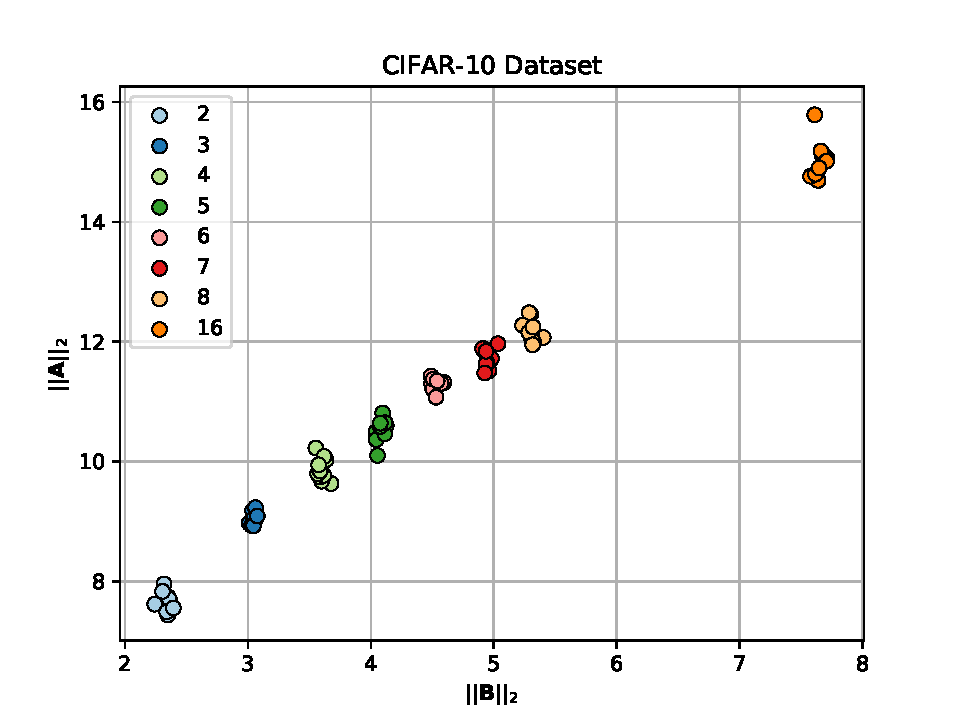
\includegraphics[width=\textwidth]{dcifstorel2norm.pdf}
  \end{subfigure}
  %\caption{Initial parameter norm $\norm{\B}_2$ vs final parameter norm $\norm{\A}_2$ with increasing depths (at width $100$) on the CIFAR-10 dataset. $10$ trials are displayed for each architecture.}
  %\label{fig:dcifstorel2norm}
  \hfill 
  \hspace{-10mm} 
  \begin{subfigure}[b]{.45\textwidth}
    \centering
  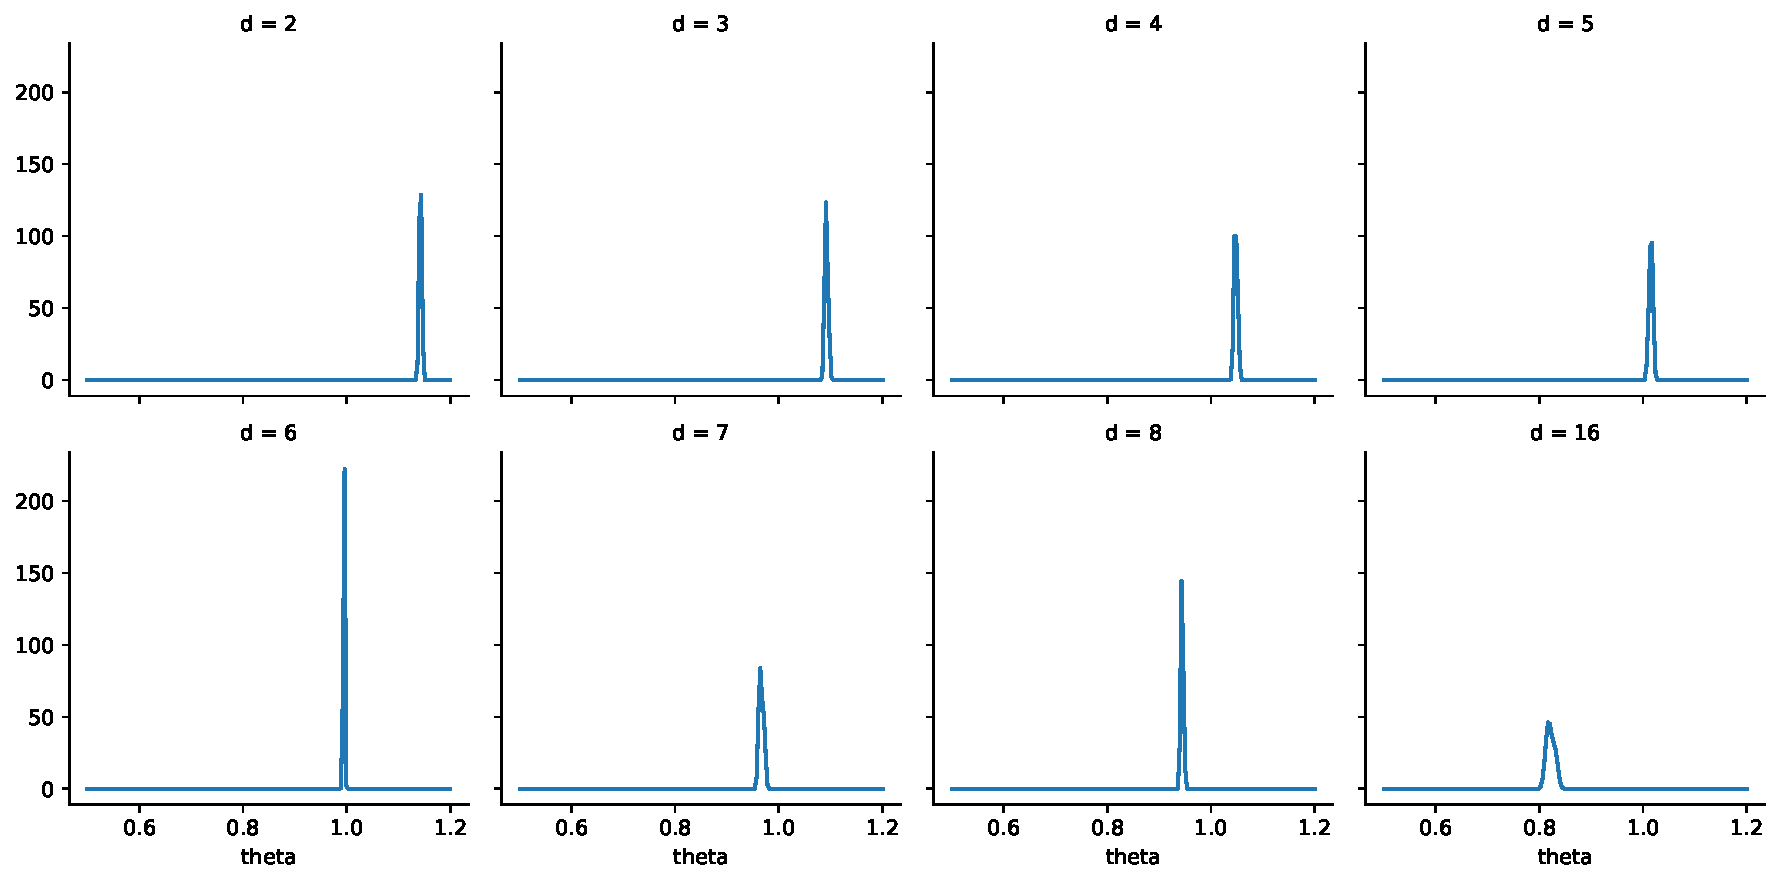
\includegraphics[width=0.95\textwidth]{dcif_kdetheta.pdf}
  %\caption{}
  %\caption{(Left) Initial parameter norm $\norm{\B}_2$ vs final parameter norm $\norm{\A}_2$ with increasing depths (at width $100$) on the CIFAR-10 dataset. $10$ trials are displayed for each architecture.  (Right) Gaussian kernel density estimate on $10$ trials of the experiment (for every depth $d$ and $100$ width) measuring the angular deviation of the weight vector under training}
  %\label{fig:dciftheta}
  \end{subfigure} 
\end{figure}

In the {\it \color{violet} figure to the right} is displayed the Gaussian kernel density estimate on $10$ trials of the experiment (at different depths and $100$ width) measuring the angular deviation of the weight vector under training. This deflection angle only decreases slightly with depth and showed negligible dependence over the widths tried. 
\vspace{2.2mm}
% \begin{figure}[htbp]
%   \centering
%   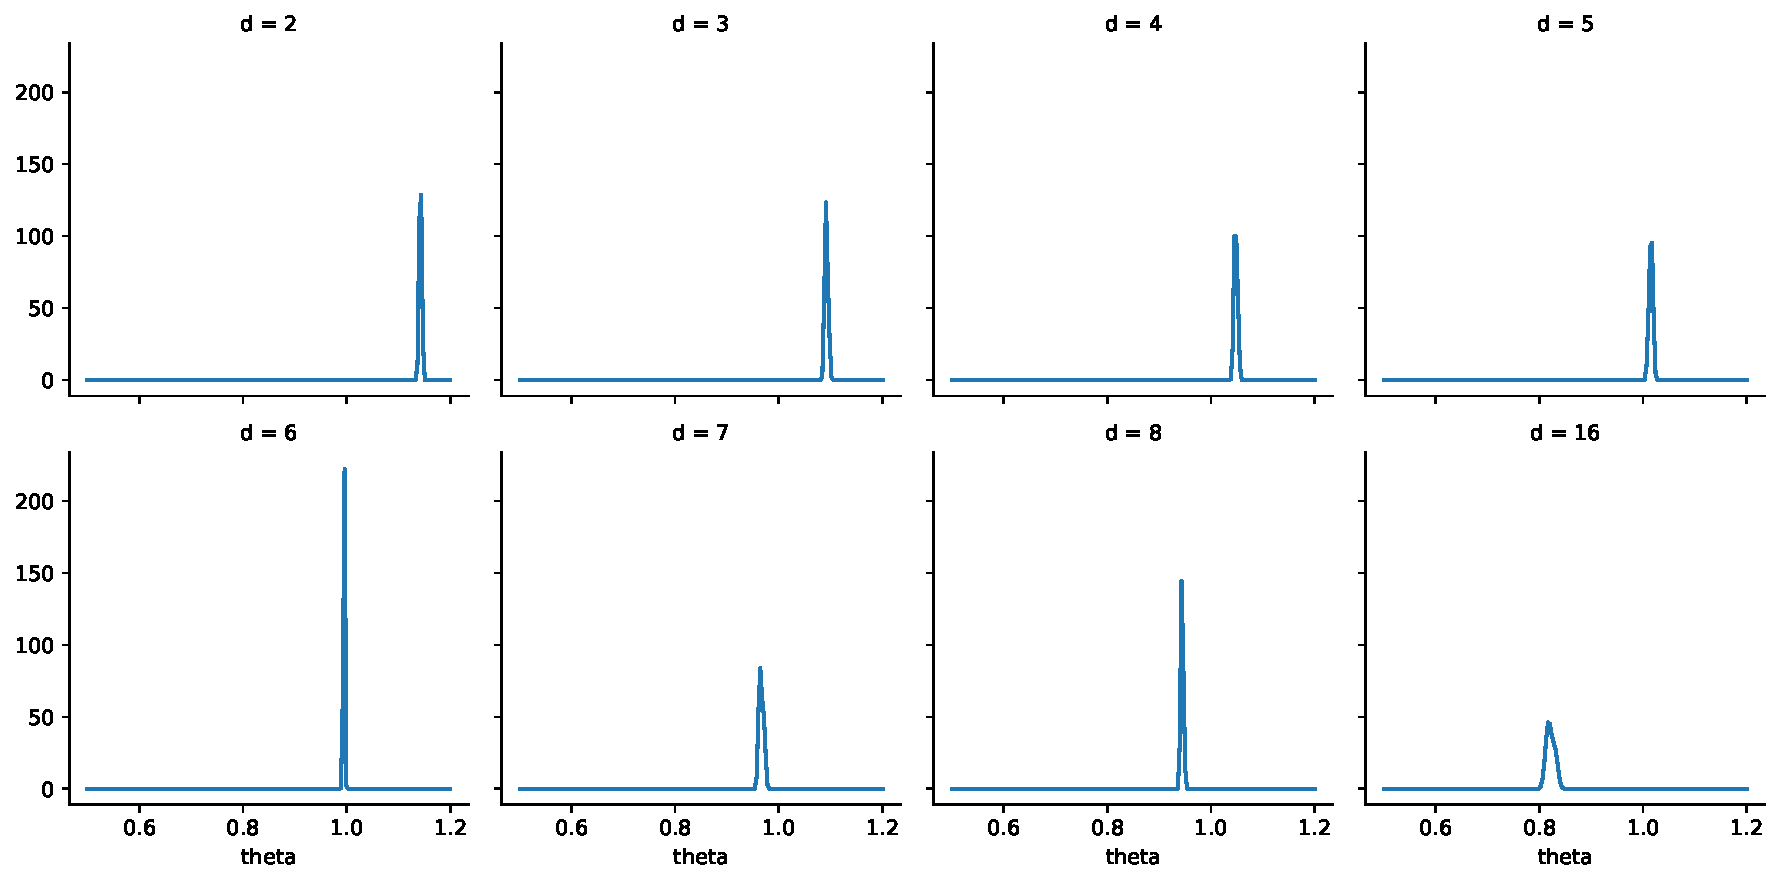
\includegraphics[width=0.5\linewidth]{dcif_kdetheta.pdf}
%   \caption{Gaussian kernel density estimate on $10$ trials of the experiment (for every depth $d$ and $100$ width) measuring the angular deviation of the weight vector under training}
%   \label{fig:dciftheta}
% \end{figure}

\end{exampleblock}


\end{column}

\end{columns}
\end{frame}

\end{document}






% \nocite{*}
% \tiny {\bibliographystyle{plainnat}}